%% Relatório final — artigo no template IEEE de conferência (IEEEtran, versão de 27/06/2024, em
%% report/IEEE-conference-template-062824/). Compilar a partir desta pasta:  pdflatex main && pdflatex main
%% As figuras são geradas por figures/make_figures.py a partir dos resultados em results/
%% (notebooks/benchmark_obstrucao.ipynb e notebooks/benchmark_manipulacao.ipynb). Os números das tabelas
%% vêm de report/resultados_benchmark_obstrucao.md e report/resultados_benchmark_manipulacao.md.
\documentclass[conference]{IEEEtran}

\usepackage[utf8]{inputenc}
\usepackage[T1]{fontenc}
\usepackage[brazil]{babel}
\usepackage{cite}
\usepackage{amsmath,amssymb,amsfonts}
\usepackage{graphicx}
\usepackage{textcomp}
\usepackage{xcolor}
\usepackage{booktabs}
\usepackage{multirow}
\usepackage{array}
\usepackage{tikz}
\usetikzlibrary{arrows.meta,positioning,calc}
\usepackage{url}
\usepackage[hidelinks]{hyperref}

\graphicspath{{figures/}}
\newcolumntype{L}[1]{>{\raggedright\arraybackslash}p{#1}}
\newcommand{\Ir}{I_r}
\newcommand{\Ia}{I_a}
\newcommand{\Ageo}{A_{\mathrm{geo}}}
\newcommand{\var}[1]{\texttt{#1}}
\newcommand{\vpaper}{\var{paper}}
\newcommand{\vneutral}{\var{neutral}}
\newcommand{\vpd}{\var{paper\_\allowbreak decomposed}}

\hyphenation{Grounding ViDDAR VIM-Sense LLaVA Qwen Gemma}
\renewcommand{\IEEEkeywordsname}{Palavras-chave}

\begin{document}

\title{Benchmark de VLMs abertos para detecção de ataques em realidade aumentada: obstrução e
manipulação de informação}

\author{\IEEEauthorblockN{Lucas Natan Correia Couri}
\IEEEauthorblockA{\textit{Centro de Informática} \\
\textit{Universidade Federal de Pernambuco}\\
Recife, Brasil \\
lncc2@cin.ufpe.br}
\and
\IEEEauthorblockN{Heitor Mendes Pereira}
\IEEEauthorblockA{\textit{Centro de Informática} \\
\textit{Universidade Federal de Pernambuco}\\
Recife, Brasil \\
hmp@cin.ufpe.br}}

\maketitle

\begin{abstract}
O ViDDAR usa modelos de visão e linguagem (VLMs) para detectar dois tipos de conteúdo de realidade
aumentada (RA) prejudicial ao usuário: a obstrução de objetos reais importantes e a manipulação da
informação que um objeto real transmite. O sistema foi avaliado com GPT-4o e LLaVA-Next-8B, e o código
publicado não reproduz os experimentos. Reconstruímos o pipeline de avaliação e apresentamos um
benchmark de cinco VLMs abertos, de 2 a 12 bilhões de parâmetros, executados localmente numa GPU de
12~GB, nas duas tarefas e nas linhas de base do artigo original. Na obstrução, em que o VLM apenas nomeia
o objeto-chave e a decisão é geométrica, o ViDDAR atinge de 84,6\% a 91,8\% de acurácia, e com dois
modelos não se distingue do pipeline que recebe o nome verdadeiro do objeto. Os poucos falsos positivos
vêm todos da escolha de outro objeto plausível em cenas ambíguas. Na manipulação, em que o VLM julga
três fatores e decide sozinho, nenhum modelo supera, com o prompt do artigo, um detector trivial que nunca
dispara (61,4\%). Para caracterizar essa falha, atribuímos cada erro a uma causa com os rótulos por fator
do dataset e testamos duas hipóteses com variantes de prompt, além de uma medida geométrica de
alinhamento. Os erros vêm de conclusões que contradizem as próprias respostas, de um viés de ``sim''
induzido pelo prompt e de percepção fraca dos fatores, e nenhum modelo distingue o fator de deturpação da
informação. Só uma das 15 configurações supera o detector trivial, e o maior ganho vem de calcular a
decisão em código a partir das respostas do próprio VLM. Nas duas tarefas, o detector funciona melhor
quando a decisão final não fica com o VLM.
\end{abstract}

\begin{IEEEkeywords}
Realidade aumentada, segurança, modelos de visão e linguagem, benchmark, falsos positivos.
\end{IEEEkeywords}

% =====================================================================================================
\section{Introdução}

Em realidade aumentada (RA), o conteúdo virtual é sobreposto à visão que o usuário tem do mundo real.
Um conteúdo mal posicionado ou malicioso pode esconder objetos importantes ou levar o usuário a
interpretar errado o que vê~\cite{roesner2014,arya}. O ViDDAR~\cite{viddar} usa modelos de visão e
linguagem (VLMs) para detectar dois tipos de conteúdo prejudicial a partir de um par de imagens, a cena
real $\Ir$ e a cena aumentada $\Ia$. A \emph{obstrução} ocorre quando o conteúdo esconde um objeto
importante, como uma placa de advertência. A \emph{manipulação de informação} ocorre quando a combinação
do conteúdo com um objeto real faz o usuário atribuir ao objeto uma função ou informação falsa. No
artigo original, o GPT-4o acerta 92,2\% dos pares de obstrução e 82,5\% dos de manipulação; com o
LLaVA-Next-8B, os números são 89,2\% e 43,0\%.

Para uso em dispositivos de RA, com restrições de privacidade, custo e latência, os candidatos naturais
são VLMs abertos e pequenos, executados localmente. Não se sabe como o ViDDAR se comporta com eles: o
artigo avalia só dois modelos, e o código publicado traz apenas demonstrações com GPT-4o. Este trabalho
responde a essa lacuna com um benchmark: reconstruímos o pipeline de avaliação do artigo e o executamos,
nas duas tarefas e com as linhas de base originais, com cinco VLMs abertos de 2 a 12 bilhões de
parâmetros, de três famílias.

Os resultados das duas tarefas são muito diferentes. Na obstrução, o ViDDAR funciona com quase todos os
modelos, e três deles passam de 90\% de acurácia. Na manipulação, nenhum modelo supera, com o prompt do
artigo, um detector trivial que nunca dispara, e a acurácia sozinha esconde o motivo: modelos com a
mesma acurácia erram em direções opostas. Por isso, a segunda parte do trabalho caracteriza as falhas da
manipulação. Usamos os rótulos por fator do dataset para atribuir cada falso positivo e cada falso
negativo a uma causa e testamos duas hipóteses sobre a origem dos erros (viés induzido pelo prompt e
conclusão desconectada das respostas), além de uma medida geométrica do alinhamento no lugar do
julgamento do VLM. O objetivo é caracterizar o problema, e não
propor um novo detector. As contribuições são:
\begin{itemize}
\item uma reimplementação aberta do pipeline de avaliação do ViDDAR e de suas linhas de base, que guarda
  as respostas brutas e permite recalcular métricas e limiares sem consultar os modelos de novo
  (\url{https://github.com/lucascouri2/viddar_rep});
\item um benchmark de cinco VLMs abertos nas duas tarefas, com testes pareados, taxas de falsos
  positivos e negativos e comparação com um detector trivial (Seções~\ref{sec:res-obs}
  e~\ref{sec:res-man});
\item a atribuição dos erros às etapas de cada pipeline e o teste de hipóteses sobre as falhas da
  manipulação, que mostram que os falsos positivos das duas tarefas têm origens diferentes
  (Seções~\ref{sec:obs-erros} a~\ref{sec:man-c2}).
\end{itemize}

% =====================================================================================================
\section{Trabalhos relacionados}
\label{sec:rel}

\textbf{Segurança da saída em RA.} Roesner \emph{et al.}~\cite{roesner2014} apontaram a saída visual
como superfície de ataque em RA, e o Arya~\cite{arya} propôs políticas que restringem o que as aplicações
podem desenhar, por exemplo, impedindo que objetos virtuais escondam pedestres. Essas políticas exigem
regras escritas à mão para cada situação. O ViDDAR~\cite{viddar} substitui as regras por um VLM que
raciocina sobre a cena, e o VIM-Sense~\cite{vimsense} estende a detecção de manipulação para vídeo,
combinando raciocínio multimodal com informações de texto e de cena. Ambos foram avaliados com modelos
comerciais e reportam principalmente acurácia.

\textbf{Vieses de VLMs e LLMs.} VLMs tendem a responder ``sim'' a perguntas sobre a presença de
objetos, e o POPE~\cite{pope} mostrou que essa tendência infla a alucinação de objetos. Modelos de
linguagem também concordam com premissas embutidas no pedido~\cite{sharma2024}, e o raciocínio passo a
passo que produzem nem sempre determina a resposta final~\cite{turpin2023}. Em avaliações feitas por
LLMs, a forma do pedido afeta o julgamento~\cite{zheng2023}, e decompor uma tarefa em subtarefas
resolvidas separadamente melhora o desempenho em problemas compostos~\cite{khot2023}. O questionário de
manipulação do ViDDAR expõe o VLM a todos esses efeitos, o que orienta as hipóteses da
Seção~\ref{sec:hipoteses}.

% =====================================================================================================
\section{O ViDDAR}
\label{sec:viddar}

O ViDDAR recebe um par de imagens do mesmo ponto de vista: $\Ir$, capturada pela câmera do dispositivo
sem o conteúdo virtual, e $\Ia$, a cena aumentada que o usuário vê. No artigo, a captura acontece no
dispositivo de RA, a detecção e a segmentação rodam num servidor de borda e o VLM roda na nuvem. Há um
pipeline para cada tipo de ataque (Fig.~\ref{fig:pipelines}).

\begin{figure*}[!t]
\centering
\begin{tikzpicture}[
  box/.style={draw=black!60, rounded corners=2pt, align=center, font=\footnotesize, fill=black!3,
              minimum height=0.95cm, inner sep=2.5pt},
  vlm/.style={box, fill=blue!8, draw=blue!55!black},
  geo/.style={box, fill=orange!10, draw=orange!60!black},
  ours/.style={box, dashed, fill=white},
  arr/.style={-{Stealth[length=1.7mm]}, black!70},
  lab/.style={font=\footnotesize\bfseries, anchor=west}]
% --- (a) obstruction
\node[lab] at (-0.1, 0.85) {(a) Obstrução};
\node[box, text width=1.25cm] (in1) at (0.75, 0) {par\\$(\Ir,\Ia)$};
\node[vlm, text width=3.3cm] (vlm1) at (3.65, 0) {\textbf{VLM} nomeia o objeto-chave em $\Ir$\\(até 4
  palavras, ex.: ``warning sign'')};
\node[geo, text width=2.2cm] (gd) at (7.05, 0) {Grounding DINO:\\caixa do objeto};
\node[geo, text width=1.6cm] (sam) at (9.45, 0) {SAM:\\máscara $m_k$};
\node[geo, text width=3.3cm] (ratio) at (12.45, 0) {obstrução se\\$|m_k\cap m_c|\,/\,|m_k|\geq\alpha$
  (Eq.~\ref{eq:obs})};
\node[box, text width=0.9cm] (o1) at (15.15, 0) {$\hat O$};
\node[geo, text width=5.6cm, minimum height=0.6cm] (mc) at (7.6, -1.15) {diferença $|\Ia-\Ir|$ +
  morfologia: máscara do conteúdo virtual $m_c$};
\draw[arr] (in1) -- node[above, font=\scriptsize]{$\Ir$} (vlm1);
\draw[arr] (vlm1) -- (gd);
\draw[arr] (gd) -- (sam); \draw[arr] (sam) -- (ratio); \draw[arr] (ratio) -- (o1);
\draw[arr] (in1.south) |- (mc.west);
\draw[arr] (mc.east) -| (ratio.south);
% --- (b) manipulation
\node[lab] at (-0.1, -2.05) {(b) Manipulação de informação};
\node[box, text width=1.25cm] (in2) at (0.75, -3.15) {par\\$(\Ir,\Ia)$};
\node[vlm, text width=5.4cm] (vlm2) at (4.75, -3.15) {\textbf{VLM} recebe $\Ir$, $\Ia$ e o questionário:
  (1) conteúdo virtual; (2) objeto-chave; (3)~$A$; (4)~$S$; (5)~$I$; (6) conclusão: ``sim'' se 3, 4 e 5
  forem ``sim''};
\node[box, text width=2.7cm] (dec) at (9.65, -3.15) {decisão: último\\``yes''/``no'' (resposta 6)};
\node[box, text width=0.9cm] (o2) at (11.85, -3.15) {$\hat M$};
\node[ours, text width=3.6cm] (fac) at (14.95, -3.15) {nossa análise: $\hat A,\hat S,\hat I$ das
  respostas 3--5, causas dos erros, $J$ por fator, regra $\hat A\wedge\hat S\wedge\hat I$};
\draw[arr] (in2) -- (vlm2); \draw[arr] (vlm2) -- (dec);
\draw[arr] (dec) -- (o2);
\draw[arr, dashed] (vlm2.south) -- ++(0,-0.3) -| (fac.south);
\end{tikzpicture}
\caption{Os dois pipelines do ViDDAR. Em azul, a etapa feita pelo VLM, que é o que o benchmark varia
(cinco modelos; na obstrução, também o prompt do objeto-chave; na manipulação, também o questionário).
Em laranja, as etapas geométricas, que não dependem do VLM. Na obstrução, o VLM só nomeia o objeto, e a
decisão é geométrica; na manipulação, o VLM percebe os três fatores e decide sozinho. O quadro tracejado
é a análise que acrescentamos sobre as respostas guardadas.}
\label{fig:pipelines}
\end{figure*}

\subsection{Detecção de obstrução}
\label{sec:viddar-obs}
Em $\Ir$ existe um conjunto de objetos-chave $K=\{k_1,\dots,k_n\}$ que não é predefinido: um objeto é
importante ou não conforme o contexto da cena. Cada $k_i$ tem uma máscara $m_k^i$, e o conteúdo virtual
tem uma máscara $m_c$. Há ataque de obstrução quando o conteúdo cobre uma fração relevante de algum
objeto-chave:
\begin{equation}
O(\Ir,\Ia)=1 \iff \exists\, k_i \in K:\; |m_k^i \cap m_c| \geq \alpha\,|m_k^i|,
\label{eq:obs}
\end{equation}
com $\alpha=0{,}25$ no artigo. O pipeline tem quatro passos (Fig.~\ref{fig:pipelines}a):
\begin{enumerate}
\item \textbf{Reconhecimento do objeto-chave.} O VLM recebe só $\Ir$ e um prompt que atribui um papel
  (``você é um especialista em observar o mundo''), pede o objeto que ``precisa da atenção das pessoas ou
  de inspeção de segurança'', dá exemplos de categorias (placas de advertência, dispositivos elétricos,
  equipamentos de segurança) e restringe a resposta a um objeto, descrito em até quatro palavras, com a
  cor se ela for relevante (``such as `red box'\,'').
\item \textbf{Localização.} O Grounding DINO~\cite{groundingdino}, um detector de vocabulário aberto,
  recebe o nome dado pelo VLM e devolve a caixa de maior escore em $\Ir$.
\item \textbf{Segmentação.} O SAM~\cite{sam} recorta, dentro dessa caixa, a máscara $m_k$ do objeto.
\item \textbf{Decisão.} A máscara $m_c$ vem da comparação pixel a pixel entre $\Ir$ e $\Ia$, e a
  Eq.~\eqref{eq:obs} decide.
\end{enumerate}
A divisão de trabalho é a ideia central do método: o VLM resolve a parte semântica (qual objeto importa
nesta cena), e a geometria resolve se ele está coberto. O artigo compara o ViDDAR com seis linhas de
base, que reproduzimos:
\begin{itemize}
\item \textbf{end-to-end}: o VLM nomeia o objeto e, numa segunda chamada com $\Ir$ e $\Ia$, responde
  ``Yes'' ou ``No'' se ele está obstruído; não há geometria;
\item \textbf{underdetailed}: o pipeline do ViDDAR com um prompt mínimo, sem papel, sem menção a
  segurança e sem exemplos;
\item \textbf{greedy}: o VLM pode listar vários objetos, e há obstrução se qualquer um passar de $\alpha$;
\item \textbf{prior knowledge}: o pipeline recebe o nome verdadeiro do objeto no lugar da resposta do
  VLM. É o limite superior do pipeline e mede o que se perde nas etapas geométricas;
\item \textbf{saliência}~\cite{hou2007} e \textbf{Canny}~\cite{canny}: sem VLM, há obstrução se a
  saliência espectral ou a densidade de bordas sob $m_c$ for maior que a média da imagem.
\end{itemize}

\subsection{Detecção de manipulação de informação}
\label{sec:viddar-man}
Para cada par formado por um objeto real $r$ e o conteúdo virtual $c$, o ViDDAR define três fatores
booleanos: \textbf{$A$}, o conteúdo está precisamente alinhado ao objeto, sem uma separação
significativa; \textbf{$S$}, o conteúdo tem textura de qualidade e estilo coerente com o mundo real; e
\textbf{$I$}, a combinação faz o usuário acreditar que o objeto tem uma função ou informação que não
tem, ou perder uma que tem. Há manipulação quando os três ocorrem juntos:
\begin{equation}
M(\Ir,\Ia)=1 \iff \exists\,(r,c):\; A \wedge S \wedge I .
\label{eq:man}
\end{equation}
A intuição é que só um conteúdo encostado no objeto, realista e semanticamente relacionado a ele engana o
usuário. Uma planta virtual flutuando acima de uma caixa de som, por exemplo, não é manipulação, porque
$A=0$ (Fig.~\ref{fig:exemplo}).

Ao contrário da obstrução, aqui o VLM faz todo o trabalho (Fig.~\ref{fig:pipelines}b). Ele recebe
$\Ir$, $\Ia$ e um questionário de seis perguntas, numa única chamada. O prompt começa afirmando que
$\Ia$ foi criada ``adicionando conteúdo virtual ao espaço''. As perguntas 1 e 2 pedem o conteúdo virtual
e o objeto-chave que interage com ele. As perguntas 3, 4 e 5 pedem ``sim'' ou ``não'' e uma explicação
para $A$, $S$ e $I$; a pergunta 5 pede para ``pensar criativamente'' e só responder ``não'' se a
combinação não tiver relação semântica específica. A pergunta 6 é a conclusão: ``se você respondeu
`sim' nas perguntas 3, 4 e 5, deve dizer `sim'; caso contrário, diga `não'\,''. A decisão do ViDDAR é a
última ocorrência de ``yes'' ou ``no'' na resposta, isto é, a resposta 6. Não há etapa geométrica: o VLM
percebe os três fatores e tira a conclusão.

\begin{figure}[!t]
\centering
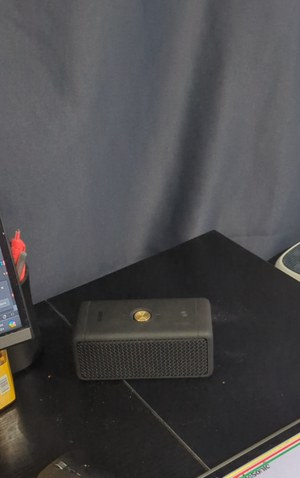
\includegraphics[width=0.31\linewidth]{ex_align_raw.jpg}\hfill
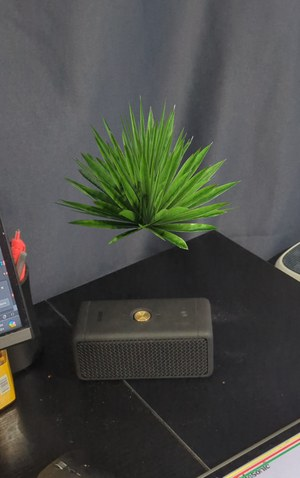
\includegraphics[width=0.31\linewidth]{ex_align_ar.jpg}\hfill
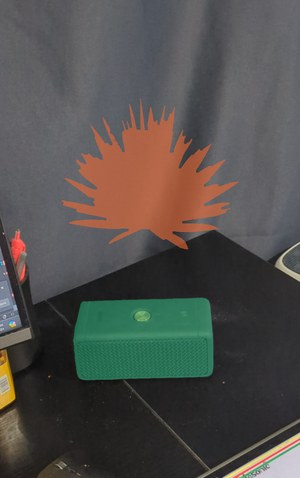
\includegraphics[width=0.31\linewidth]{ex_align_masks.jpg}
\caption{Par benigno do dataset de manipulação ($A=0$, $S=1$, $I=1$, $M=0$). Esquerda: $\Ir$. Centro:
$\Ia$, com uma planta virtual acima da caixa de som. Direita: o componente geométrico da
Seção~\ref{sec:hipoteses}, com o objeto detectado a partir do nome dado pelo Qwen3-VL-4B (verde) e o
conteúdo extraído pela diferença entre as imagens (laranja). A separação de 142 pixels indica $A=0$; o
VLM havia respondido que o conteúdo estava alinhado. Recortes das imagens originais.}
\label{fig:exemplo}
\end{figure}

% =====================================================================================================
\section{Metodologia do benchmark}
\label{sec:metodo}

\subsection{Reconstrução do pipeline}
\label{sec:reconstrucao}
O repositório dos autores traz o dataset e dois notebooks de demonstração com GPT-4o, mas não o código
que produz os resultados do artigo. Os notebooks divergem do artigo em pontos que afetam o resultado (o
de obstrução sorteia $\alpha$ entre 0,175 e 0,225 a cada imagem e usa outro prompt), e faltam as linhas
de base, as métricas de reconhecimento e segmentação e a geração das máscaras $m_c$; o dataset publica só
32 dessas máscaras, sem indicar a que pares pertencem.

Reimplementamos o pipeline seguindo o artigo: os prompts são transcritos literalmente, a
Eq.~\eqref{eq:obs} usa o mesmo $\alpha$ e a decisão da manipulação é o último ``yes''/``no''. Há duas
diferenças por necessidade: o Grounding DINO aberto no lugar da versão~1.5, disponível só por API, e os
VLMs abertos no lugar dos modelos acessados por API. Onde o artigo é omisso, tomamos decisões explícitas.
A máscara $m_c$ é a região em que algum canal de cor difere mais de 30 níveis entre $\Ir$ e $\Ia$, seguida
de abertura e fechamento morfológicos; ela tem IoU mediano de 0,99 com as 32 máscaras publicadas. Os
fatores $\hat A$, $\hat S$ e $\hat I$ são lidos da primeira ocorrência de ``yes''/``no'' nas respostas 3,
4 e 5. Uma resposta que não pode ser interpretada conta como erro e nunca é descartada. O código guarda a
resposta bruta do VLM, a razão de obstrução e as respostas por fator, de modo que limiares, regras de
decisão e métricas são recalculados sem consultar os modelos de novo.

\subsection{Modelos e execução}
Avaliamos cinco VLMs abertos de três famílias: Qwen3-VL-2B, -4B e -8B (Instruct)~\cite{qwen3vl}, que
mostram o efeito do tamanho dentro de uma família; LLaVA-Next-8B~\cite{llava}
(\texttt{llama3-llava-next-8b}), o mesmo modelo do artigo; e Gemma~4 12B~\cite{gemma4}. Todos rodam
localmente numa GPU NVIDIA RTX 3060 de 12~GB, o 2B e o 4B em bf16 e os três maiores quantizados em 4 bits
(NF4~\cite{qlora}). A decodificação é greedy (temperatura 0), as imagens são reduzidas a no máximo 1
megapixel e passadas na ordem $\Ir$, $\Ia$, e a resposta é limitada a 768 tokens. O segmentador é o SAM
ViT-B, como no artigo. Na obstrução, o VLM leva de 1 a 3~s por amostra, e a geometria, 0,8~s; na
manipulação, o questionário leva de 13 a 23~s por par.

\subsection{Dados}
O dataset de obstrução tem 306 pares de 23 classes de objeto-chave (placas, extintores, tomadas, facas,
entre outras), com 3 a 29 pares por classe; 145 são obstruídos. O de manipulação tem 114 pares com
rótulos de $A$, $S$, $I$ e $M$ que satisfazem a Eq.~\eqref{eq:man}: 44 ataques e 70 benignos, dos quais
32 têm só $A$ falso, 25 só $S$, 11 só $I$ e 2 têm $A$ e $S$ falsos. Dois pontos pesam na análise: um
detector que nunca dispara acerta 61,4\% dos pares, e só 11 benignos testam a rejeição de $I$.

\subsection{Métricas e testes}
Reportamos as métricas do artigo (acurácia, precisão e recall) e acrescentamos a taxa de falsos
positivos (FPR, fração dos benignos marcados como ataque), que é o foco da análise. Na manipulação,
reportamos também a taxa de falsos negativos (FNR, fração dos ataques perdidos, igual a $1-$recall),
porque é nela que aparecem os modelos que quase nunca disparam. Num gráfico de recall contra FPR, um
detector que ignora a entrada fica sobre a diagonal $\text{recall}=\text{FPR}$, e o detector trivial
que nunca dispara fica na origem. Os intervalos de 95\% são de Wilson~\cite{wilson}. Duas execuções são
comparadas nos mesmos pares pelo teste exato de McNemar bilateral~\cite{mcnemar1947,dietterich1998}, que
usa só os pares em que exatamente uma delas acerta; uma diferença só conta com $p<0{,}05$. Na
manipulação, cada execução é comparada também com o detector trivial.

Na obstrução, o objeto-chave conta como reconhecido quando a máscara recortada a partir da frase do VLM
tem IoU $\geq 0{,}5$ com a máscara verdadeira; comparar só o texto seria permissivo demais (``black tv
stand'' contaria como TV). Na manipulação, medimos quanto a resposta do VLM sobre cada fator
$F\in\{A,S,I\}$ informa sobre o rótulo pelo índice de Youden~\cite{youden1950}:
\begin{equation}
J_F = P(\hat F=\text{sim}\mid F=1) - P(\hat F=\text{sim}\mid F=0).
\label{eq:youden}
\end{equation}
$J_F=0$ quando a resposta não depende do rótulo, como num modelo que sempre diz ``sim'', e $J_F=1$ para um
juiz perfeito. Ao contrário da acurácia por fator, $J_F$ não premia o viés para o rótulo majoritário.

\subsection{Atribuição de erros}
\label{sec:atrib}
\textbf{Obstrução.} Cada erro do ViDDAR é atribuído à etapa que falhou: \emph{nada detectado}, quando o
Grounding DINO não encontra o nome; \emph{objeto errado}, quando a máscara recortada tem IoU $<0{,}5$ com
a verdadeira; e \emph{limiar}, quando o objeto certo foi recortado, mas a razão ficou do lado errado de
$\alpha$. Se o \emph{prior knowledge} acerta a mesma amostra, o erro é do VLM; se também erra, o
problema está depois do VLM.

\textbf{Manipulação.} Como o dataset rotula os três fatores, cada erro recebe uma causa, nesta ordem:
\emph{ilegível}, quando a decisão ou alguma resposta 3--5 não pôde ser interpretada; \emph{conclusão},
quando $\hat A\wedge\hat S\wedge\hat I$ leva a uma decisão e a resposta 6 diz o contrário; e
\emph{percepção}, quando a conclusão segue as respostas e o erro está nos fatores. Num falso positivo, o
modelo aceitou os fatores cujo rótulo é 0; num falso negativo, rejeitou algum fator, todos com rótulo 1.
Cada causa é contada sobre os pares em que pode ocorrer: aceitar um $A$ falso, por exemplo, só pode
acontecer nos 32 benignos cujo único fator falso é $A$.

\subsection{Hipóteses sobre as falhas da manipulação}
\label{sec:hipoteses}
A literatura da Seção~\ref{sec:rel} sugere duas origens para os erros, e cada uma deu origem a uma
variante do prompt. As variantes foram escritas a partir do prompt e das definições do próprio artigo,
e não dos pares em que os modelos erraram, e foram congeladas antes das execuções completas. O prompt do
artigo é a variante \vpaper\ (P).
\begin{itemize}
\item \textbf{H1, viés induzido pelo prompt} (\vneutral, N): o prompt afirma que há conteúdo virtual e
  pede para ``pensar criativamente'', o que empurraria o modelo para o ``sim''. A variante diz que $\Ia$
  ``pode conter'' conteúdo virtual e retira a instrução.
\item \textbf{H2, conclusão desconectada e contaminação entre respostas} (\vpd, PD): uma chamada pede o
  conteúdo e o objeto (até 4 palavras cada), e uma chamada por fator repete a pergunta 3, 4 ou 5,
  citando o conteúdo e o objeto. A decisão $\hat A\wedge\hat S\wedge\hat I$ é calculada em código, o que
  elimina por construção o erro de conclusão. Para separar os dois efeitos, aplicamos a mesma regra às
  respostas 3--5 do questionário conjunto, sem nova consulta ao modelo.
\end{itemize}
\textbf{C2, alinhamento geométrico.} O fator $A$ é o mais geométrico dos três, e por isso testamos se uma
medida em pixels julga melhor que o VLM. Reaproveitamos os componentes da obstrução: o nome do objeto
dado pelo VLM vai para o Grounding DINO e o SAM, que produzem $m_k$, e $m_c$ vem da diferença entre as
imagens (Fig.~\ref{fig:exemplo}). A medida é a menor distância entre $m_c$ e $m_k$, dividida pelo maior
lado da caixa de $m_c$, e $\Ageo=1$ quando ela fica abaixo de um limiar escolhido por validação cruzada
estratificada em 5 partições. A decisão híbrida é $\Ageo\wedge\hat S\wedge\hat I$, aplicada às
respostas do prompt \vpaper.

% =====================================================================================================
\section{Resultados: obstrução}
\label{sec:res-obs}

\begin{table}[!t]
\renewcommand{\arraystretch}{1.05}
\caption{Detecção de obstrução nos 306 pares (\%), com $\alpha=0{,}25$. Em negrito, o melhor valor de
cada linha}
\label{tab:obs}
\centering
\footnotesize
\setlength{\tabcolsep}{3.5pt}
\begin{tabular}{lccccc}
\toprule
 & Qwen 2B & Qwen 4B & Qwen 8B & LLaVA & Gemma \\
\midrule
\multicolumn{6}{l}{\textit{ViDDAR}} \\
\quad acurácia & 84,6 & 91,5 & \textbf{91,8} & 88,2 & 90,5 \\
\quad \scriptsize IC 95\% & \scriptsize 80--88 & \scriptsize 88--94 & \scriptsize 88--94 & \scriptsize 84--91 & \scriptsize 87--93 \\
\quad precisão & 90,8 & 95,4 & \textbf{97,6} & 91,6 & 97,5 \\
\quad recall & 75,2 & \textbf{86,2} & 84,8 & 82,8 & 82,1 \\
\quad FPR & 6,8 & 3,7 & \textbf{1,9} & 6,8 & \textbf{1,9} \\
\quad objeto-chave & 72,5 & \textbf{89,9} & 85,0 & 76,1 & 88,6 \\
\midrule
\multicolumn{6}{l}{\textit{End-to-end}} \\
\quad acurácia & 45,1 & 72,9 & 73,5 & 51,3 & \textbf{81,7} \\
\quad recall & 81,4 & 66,9 & \textbf{84,8} & 8,3 & 80,7 \\
\quad FPR & 87,6 & 21,7 & 36,6 & \textbf{9,9} & 17,4 \\
\midrule
\multicolumn{6}{l}{\textit{Demais linhas de base (acurácia)}} \\
\quad underdetailed & 82,7 & \textbf{85,6} & 82,7 & 82,7 & 80,1 \\
\quad greedy & 88,9 & 90,5 & \textbf{92,2} & 87,3 & 90,5 \\
\quad prior knowledge & \multicolumn{5}{c}{93,8 (sem VLM)} \\
\quad saliência / Canny & \multicolumn{5}{c}{52,3 / 49,7 (sem VLM)} \\
\bottomrule
\multicolumn{6}{L{8.2cm}}{\scriptsize Objeto-chave: fração dos pares em que a máscara recortada a
partir da frase do VLM tem IoU $\geq 0{,}5$ com a verdadeira.}
\end{tabular}
\end{table}

\subsection{Desempenho e replicação}
A Tabela~\ref{tab:obs} traz o benchmark. Antes de comparar modelos, conferimos a reconstrução com os
números publicados. Os métodos sem VLM validam detector, segmentador, $m_c$ e Eq.~\eqref{eq:obs}: o
\emph{prior knowledge} tem 93,8\% contra 93,1\% no artigo, e saliência e Canny ficam perto do acaso,
como no original. Com o LLaVA-Next-8B, o mesmo VLM do artigo, o ViDDAR tem 88,2\% contra 89,2\%, e o
end-to-end, 51,3\% contra 55,2\%.

Com o ViDDAR, todos os modelos ficam entre 84,6\% e 91,8\%. O Qwen3-VL-4B, o Qwen3-VL-8B e o Gemma~4
passam de 90\% e empatam entre si no McNemar ($p\geq 0{,}39$). O 4B e o 8B também não se distinguem do
\emph{prior knowledge} ($p=0{,}065$ e $0{,}15$): com eles, o reconhecimento do objeto-chave deixa de ser
o gargalo do pipeline. O Qwen3-VL-2B perde para os três e para o \emph{prior} ($p\leq 0{,}001$), por
reconhecer o objeto certo em só 72,5\% dos pares. Na família Qwen, o tamanho ajuda do 2B para o 4B
(+6,9 pontos), mas não do 4B para o 8B (6 contra 7 pares discordantes, $p=1{,}0$). O detector erra mais
por omissão que por alarme falso: a precisão vai de 90,8\% a 97,6\% e a FPR fica abaixo de 7\%, mas o
recall fica entre 75,2\% e 86,2\%.

\subsection{Separar reconhecimento e decisão}
O ViDDAR supera o end-to-end nos cinco modelos, com ganhos de 8,8 a 39,5 pontos ($p\leq 0{,}001$ em
todos), o que confirma a tese central do artigo também com VLMs abertos. Quando o VLM decide sozinho, cada
modelo mostra um viés próprio: o Qwen3-VL-2B diz ``obstruído'' em 259 das 306 amostras (FPR de 87,6\%),
o LLaVA em apenas 28 (recall de 8,3\%), o 8B tende ao ``sim'' e o 4B, ao ``não''. Só o Gemma~4 é
equilibrado: diz ``sim'' em 145 amostras, exatamente o número de obstruídas, e tem o melhor end-to-end
(81,7\%). Esses mesmos vieses reaparecem na manipulação (Seção~\ref{sec:res-man}).

\subsection{O prompt do objeto-chave}
O \emph{underdetailed} piora quatro dos cinco modelos, de 5,5 a 10,4 pontos ($p\leq 0{,}012$), como no
artigo. Sem a orientação de segurança, os modelos nomeiam objetos salientes, mas irrelevantes: ``door''
é a resposta mais frequente do Gemma~4 (29 vezes) e do 2B (27), e o reconhecimento do Gemma~4 cai de
88,6\% para 62,1\%. O papel e os exemplos do prompt dizem \emph{que tipo} de objeto importa, e é isso que
define o objeto-chave. O \emph{greedy} empata com o ViDDAR em quase todos os modelos; só o 2B melhora
(84,6\% para 88,9\%, $p=0{,}007$), porque listar vários objetos compensa a má escolha de um único.

\subsection{De onde vêm os erros}
\label{sec:obs-erros}

\begin{table}[!t]
\renewcommand{\arraystretch}{1.05}
\caption{Erros do ViDDAR por etapa do pipeline. Entre parênteses, quantas dessas amostras o \emph{prior
knowledge} também erra}
\label{tab:obs-causas}
\centering
\footnotesize
\setlength{\tabcolsep}{3.2pt}
\begin{tabular}{llccccc}
\toprule
Erro & Etapa & 2B & 4B & 8B & LLaVA & Gemma \\
\midrule
FP & objeto errado & 11 (0) & 6 (0) & 3 (0) & 11 (0) & 3 (0) \\
\midrule
\multirow{3}{*}{FN} & nada detectado & 3 (0) & 0 & 0 & 0 & 0 \\
 & objeto errado & 17 (2) & 5 (3) & 7 (2) & 15 (6) & 12 (4) \\
 & limiar & 16 (14) & 15 (14) & 15 (14) & 10 (9) & 14 (13) \\
\bottomrule
\multicolumn{7}{l}{\scriptsize O \emph{prior knowledge} tem 1 FP e 18 FN, dos quais 16 de limiar.}
\end{tabular}
\end{table}

A Tabela~\ref{tab:obs-causas} atribui cada erro a uma etapa.

\textbf{Falsos positivos: qual objeto importa.} Os falsos positivos são raros (FPR de 1,9\% a 6,8\%) e
todos de reconhecimento: em cada um, o VLM nomeia um objeto diferente do anotado, e o conteúdo virtual
cobre esse outro objeto. O \emph{prior knowledge} acerta todas essas amostras. Os casos se concentram em
cenas com mais de um objeto plausível (Fig.~\ref{fig:obs-fp}). Em \emph{warning sign}, quatro modelos
nomeiam a porta onde está a placa (``black door with sign'') ou um poste amarelo próximo; em
\emph{boiling pot}, quatro modelos nomeiam o queimador ou o próprio fogão (``glowing red burner'',
``black stove''). Fora dessas classes e de \emph{electrical outlet}, o 4B, o 8B e o Gemma~4 têm só 2
falsos positivos somados. No 2B, 5 dos 11 vêm de ``red box'', cópia do exemplo do prompt e a resposta
mais frequente desse modelo (36 vezes), numa classe que não existe no dataset. Os falsos positivos da
obstrução, portanto, não vêm de erro de percepção visual nem da geometria, e sim de uma escolha que o
prompt não especifica: em cenas ambíguas, o VLM escolhe um candidato razoável diferente do anotado.

\begin{figure}[!t]
\centering
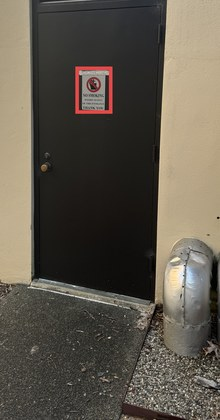
\includegraphics[height=2.75cm]{ex_fp_warning-sign_002_raw.jpg}\hspace{1pt}%
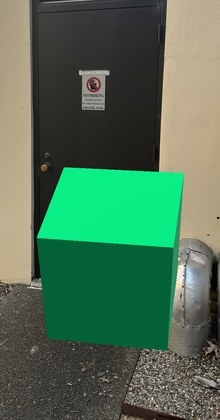
\includegraphics[height=2.75cm]{ex_fp_warning-sign_002_ar.jpg}\hfill
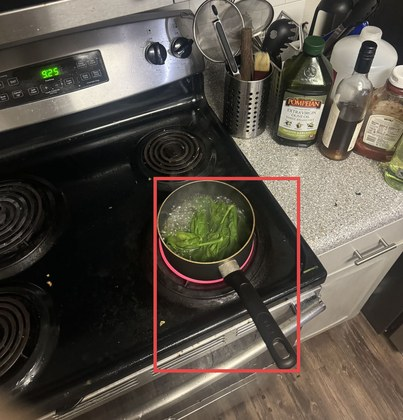
\includegraphics[height=2.75cm]{ex_fp_boiling-pot_010_raw.jpg}\hspace{1pt}%
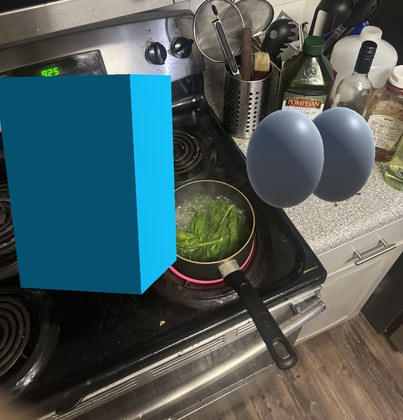
\includegraphics[height=2.75cm]{ex_fp_boiling-pot_010_ar.jpg}
\caption{Dois pares não obstruídos que quatro dos cinco VLMs marcam como obstruídos. Em cada par, à
esquerda, $\Ir$ com o objeto-chave anotado (contorno vermelho) e, à direita, $\Ia$. Esquerda: a placa de
advertência; os modelos nomeiam a porta (``black door with sign''), coberta em 41\% pelo cubo virtual.
Direita: a panela fervendo; os modelos nomeiam o queimador ou o fogão (``glowing red burner'', ``black
stove''), cobertos em 25\% a 47\%. Recortes das imagens originais.}
\label{fig:obs-fp}
\end{figure}

\textbf{Falsos negativos: cobertura logo abaixo de $\alpha$.} Os falsos negativos são o erro dominante
(FNR de 13,8\% a 24,8\%). Os de limiar são de 10 a 16 por modelo: o objeto certo foi recortado, mas a
cobertura ficou entre 0,06 e 0,249, com mediana de cerca de 0,21. O \emph{prior knowledge} erra de 9 a
14 deles, e 7 se repetem nos cinco modelos: são um limite do limiar, da máscara $m_c$ ou do rótulo, e não
do VLM. Coerentemente, todas as curvas de acurácia em função de $\alpha$, inclusive a do \emph{prior},
têm o pico em $\alpha=0{,}20$, com 1,0 a 2,0 pontos acima de $\alpha=0{,}25$ (o 4B e o 8B chegam a 93,5\%).
A explicação provável é que as nossas máscaras $m_c$ sejam um pouco menores que as dos autores.
Mantivemos $\alpha=0{,}25$, porque escolher o limiar no conjunto de teste seria otimista; a ordem dos
modelos não muda com $\alpha$. Os falsos negativos de objeto errado são, na maioria, erros do VLM
(``orange spray bottle'' no lugar da TV); alguns são do detector, como nas amostras de semáforo, em que
todos os modelos dizem ``red traffic light'', mas o semáforo segmentado não é o anotado, inclusive no
\emph{prior}.

% =====================================================================================================
\section{Resultados: manipulação de informação}
\label{sec:res-man}

\begin{table*}[!t]
\renewcommand{\arraystretch}{1.0}
\caption{Detecção de manipulação nos 114 pares (\%), com as três variantes de prompt da
Seção~\ref{sec:hipoteses}. ``vs.~P'': diferença de acurácia para o prompt do artigo e $p$ do
McNemar. ``vs.~trivial'': comparação com o detector que nunca dispara (61,4\%), pelo McNemar. $J$:
índice de Youden de cada fator (Eq.~\ref{eq:youden})}
\label{tab:man}
\centering
\footnotesize
\setlength{\tabcolsep}{4.2pt}
\begin{tabular}{llcccccccccc}
\toprule
Modelo & Variante & Acurácia & Precisão & Recall & FPR & FNR & vs.~P ($p$) & vs.~trivial & $J_A$ & $J_S$ & $J_I$ \\
\midrule
\multirow{3}{*}{Qwen3-VL-2B}
 & P  & 38,6 & 38,2 & 95,5 & 97,1 & 4,5 & -- & abaixo & $-$0,03 & $-$0,02 & 0,00 \\
 & N  & 48,2 & 42,7 & 93,2 & 78,6 & 6,8 & +9,6 (0,019) & n.s. & $-$0,03 & $-$0,01 & 0,00 \\
 & PD & 37,7 & 37,4 & 90,9 & 95,7 & 9,1 & $-$0,9 (n.s.) & abaixo & $-$0,03 & 0,07 & 0,00 \\
\midrule
\multirow{3}{*}{Qwen3-VL-4B}
 & P  & 61,4 & 50,0 & 6,8 & 4,3 & 93,2 & -- & n.s. & 0,09 & 0,31 & $-$0,30 \\
 & N  & 61,4 & -- & 0,0 & 0,0 & 100 & 0,0 (n.s.) & n.s. & 0,28 & 0,41 & $-$0,20 \\
 & PD & 73,7 & 93,8 & 34,1 & 1,4 & 65,9 & +12,3 (0,003) & \textbf{acima} & 0,25 & 0,22 & $-$0,01 \\
\midrule
\multirow{3}{*}{Qwen3-VL-8B}
 & P  & 37,7 & 38,1 & 97,7 & 100 & 2,3 & -- & abaixo & 0,48 & 0,25 & $-$0,01 \\
 & N  & 60,5 & 49,4 & 90,9 & 58,6 & 9,1 & +22,8 ($<$0,001) & n.s. & 0,48 & 0,22 & 0,08 \\
 & PD & 69,3 & 61,5 & 54,5 & 21,4 & 45,5 & +31,6 ($<$0,001) & n.s. & 0,32 & 0,50 & $-$0,09 \\
\midrule
\multirow{3}{*}{LLaVA-Next-8B}
 & P  & 38,6 & 37,0 & 84,1 & 90,0 & 15,9 & -- & abaixo & $-$0,13 & $-$0,02 & 0,00 \\
 & N  & 53,5 & 42,6 & 59,1 & 50,0 & 40,9 & +14,9 (0,014) & n.s. & 0,05 & $-$0,03 & 0,00 \\
 & PD & 63,2 & 55,0 & 25,0 & 12,9 & 75,0 & +24,6 (0,003) & n.s. & 0,05 & $-$0,06 & 0,00 \\
\midrule
\multirow{3}{*}{Gemma 4 12B}
 & P  & 55,3 & 46,2 & 95,5 & 70,0 & 4,5 & -- & n.s. & 0,20 & 0,16 & 0,25 \\
 & N  & 59,6 & 48,2 & 61,4 & 41,4 & 38,6 & +4,4 (n.s.) & n.s. & 0,24 & 0,31 & 0,18 \\
 & PD & 61,4 & -- & 0,0 & 0,0 & 100 & +6,1 (n.s.) & n.s. & 0,35 & 0,00 & 0,21 \\
\midrule
\bottomrule
\multicolumn{12}{l}{\scriptsize Precisão indefinida (--) quando o modelo nunca dispara. O $J_I$ usa só os 11 pares com $I=0$ e é pouco preciso.}
\end{tabular}
\end{table*}

\begin{figure*}[!t]
\centering
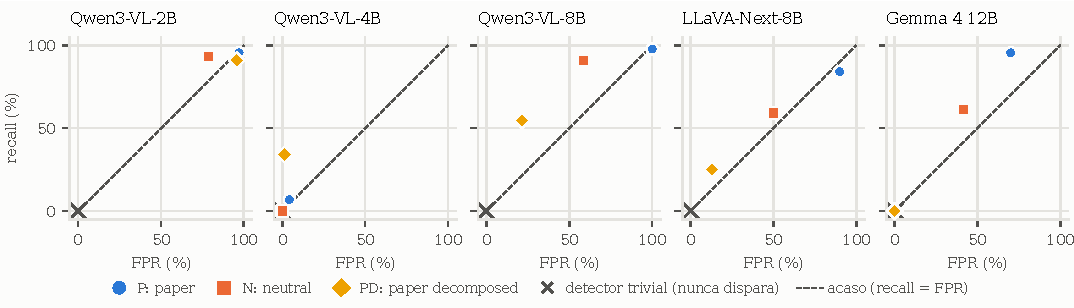
\includegraphics[width=\textwidth]{fig_op.pdf}
\caption{Recall contra FPR de cada variante na manipulação. O canto superior esquerdo é o ideal; a
diagonal tracejada é o desempenho de um detector que ignora a entrada, e o $\times$, na origem, é o
detector trivial que nunca dispara (no Qwen3-VL-4B com N e no Gemma~4 com PD, o ponto coincide com
ele). Com o prompt do artigo (P), quatro modelos ficam sobre a diagonal, e só o Gemma~4 fica acima
dela. N e PD, em geral, deslocam o ponto ao longo da diagonal, trocando falsos positivos por falsos
negativos; só os decompostos do 4B e do 8B se afastam dela.}
\label{fig:op}
\end{figure*}

\subsection{Desempenho geral}
A Tabela~\ref{tab:man} traz as 15 execuções, e a Fig.~\ref{fig:op}, o recall e a FPR de cada uma.
\textbf{Com o prompt do artigo, nenhum modelo supera o detector trivial.} O Qwen3-VL-2B, o 8B e o LLaVA
disparam em 90\% a 100\% dos benignos e ficam significativamente abaixo dele; o 4B quase nunca dispara e
o empata; o Gemma~4 fica em 55,3\%. O LLaVA (38,6\%) reproduz de perto o artigo (43,0\%), com o mesmo
padrão de recall alto e precisão baixa. Quatro dos cinco pontos ficam sobre a diagonal da
Fig.~\ref{fig:op}: esses modelos detectam ataques e disparam em benignos na mesma proporção, como um
detector que ignora a entrada. Só o Gemma~4 fica acima dela (recall de 95,5\% com FPR de 70\%).

Quase todo ganho de acurácia das variantes troca falsos positivos por falsos negativos: o LLaVA
decomposto sobe para 63,2\%, mas o recall cai de 84\% para 25\%. Como há mais benignos que ataques,
deslocamentos para o ``não'' aumentam a acurácia e saem significativos contra \vpaper\ sem melhorar a
discriminação; por isso, a comparação com o detector trivial é mais informativa que a acurácia.
\textbf{Só 1 das 15 execuções supera o detector trivial}: o Qwen3-VL-4B decomposto (73,7\%), que detecta
15 dos 44 ataques com 1 alarme falso (precisão de 93,8\%, recall de 34,1\%). O Qwen3-VL-8B decomposto é o
detector mais equilibrado (69,3\%, recall de 54,5\%, FPR de 21,4\%), mas não se distingue do trivial
($p=0{,}20$).

\subsection{Causas dos erros com o prompt do artigo}
\label{sec:man-causas}

\begin{table}[!t]
\renewcommand{\arraystretch}{1.05}
\caption{Causas dos erros com o prompt do artigo: erros sobre o número de pares em que a causa pode
ocorrer. ``Aceitou'' e ``rejeitou'' se referem às respostas 3--5}
\label{tab:causas}
\centering
\footnotesize
\setlength{\tabcolsep}{2.6pt}
\begin{tabular}{llccccc}
\toprule
 & Causa & 2B & 4B & 8B & LLaVA & Gemma \\
\midrule
\multirow{5}{*}{FP} & conclusão & 68/70 & 0/70 & 44/70 & 0/70 & 0/70 \\
 & aceitou $A$ & 0/32 & 2/32 & 10/32 & 31/32 & 22/32 \\
 & aceitou $S$ & 0/25 & 1/25 & 11/25 & 22/25 & 18/25 \\
 & aceitou $I$ & 0/11 & 0/11 & 5/11 & 8/11 & 7/11 \\
 & aceitou $A$+$S$ & 0/2 & 0/2 & 0/2 & 2/2 & 2/2 \\
\midrule
\multirow{3}{*}{FN} & rejeitou $I$ & 0/44 & 38/44 & 0/44 & 0/44 & 0/44 \\
 & rejeitou $A$ e/ou $S$ & 0/44 & 3/44 & 1/44 & 7/44 & 1/44 \\
 & ilegível ou conclusão & 2/44 & 0/44 & 0/44 & 0/44 & 1/44 \\
\midrule
\multicolumn{2}{l}{Total FP / FN} & 68 / 2 & 3 / 41 & 70 / 1 & 63 / 7 & 49 / 2 \\
\bottomrule
\end{tabular}
\end{table}

A Tabela~\ref{tab:causas} mostra que não há uma causa comum:
\begin{itemize}
\item \textbf{Conclusão desconectada (Qwen3-VL-2B e 8B).} No 2B, 68 dos 70 falsos positivos são de
  conclusão: o modelo responde ``não'' a $I$ em todos os pares e, mesmo assim, conclui ``sim'' em 96\%
  deles. O 8B responde ``Yes.'' à pergunta 6 em 113 dos 114 pares, mesmo depois de ``No'' nas perguntas 3
  ou 4: ``\emph{3. No. The virtual plant is positioned floating in the air directly above the hard drive,
  with a clear gap [\dots] 6. Yes.}''
\item \textbf{Aceitação de alinhamento e estilo ruins (LLaVA e Gemma~4).} A conclusão é coerente, mas os
  modelos aceitam $A$ em 31 e 22 dos 32 pares desalinhados e $S$ em 22 e 18 dos 25 com estilo falso.
\item \textbf{Leitura restritiva de $I$ (Qwen3-VL-4B).} 38 dos 41 falsos negativos vêm da rejeição de $I$
  em ataques: o modelo considera inofensivas adições plausíveis.
\end{itemize}

\textbf{Os modelos percebem os fatores?} As colunas $J$ da Tabela~\ref{tab:man} respondem. No 2B e no
LLaVA, $|J|\leq 0{,}13$ em todos os fatores e variantes: as respostas não dependem da imagem, e as
variantes só deslocam o viés. Na família Qwen, o tamanho melhora a percepção de $A$ e $S$: $J_A$ vai de
$-0{,}03$ (2B) a 0,09 (4B) e 0,48 (8B). \textbf{Nenhum modelo distingue $I$}: $J_I$ fica entre $-0{,}30$ e
$0{,}25$ nas 15 execuções, e só o Gemma~4 tem valores positivos em todas as variantes, com intervalos
largos. Como $I=1$ em 103 dos 114 pares, dizer sempre ``sim'' a $I$ é a estratégia que mais acerta, e as
variantes que melhoram o resultado fazem exatamente isso. Na prática, o detector se reduz a $A\wedge S$.

\subsection{Teste das hipóteses}
\label{sec:man-hip}
\textbf{H1, viés induzido pelo prompt: confirmada nos modelos que disparam demais.} Com \vneutral, a FPR
cai em todos os modelos com viés de ``sim'': de 97\% para 79\% no 2B, de 100\% para 59\% no 8B, de 90\%
para 50\% no LLaVA e de 70\% para 41\% no Gemma~4. A acurácia sobe com significância no 2B, no 8B e no
LLaVA. Nos modelos que não percebem os fatores, porém, a queda de falsos positivos vira aumento de falsos
negativos: no Gemma~4, a FNR sobe de 4,5\% para 38,6\%, e a acurácia não muda significativamente.

\textbf{H2, conclusão desconectada e contaminação: confirmada em parte.} Decompor elimina os erros de
conclusão e dá os maiores ganhos entre as variantes: +12,3 pontos no 4B, +31,6 no 8B e +24,6 no LLaVA
(este à custa do recall). No lugar da conclusão, aparece o viés de cada pergunta isolada. O 4B e o
Gemma~4 passam a rejeitar $S$; o Gemma descreve o conteúdo como ``\emph{a 2D sticker placed over the
image}'' em todos os pares e vira um detector que nunca dispara. O LLaVA passa a rejeitar $A$ nos
ataques (28 de 44), e o 2B não muda: perguntado um fator de cada vez, diz ``sim'' a $A$ em 98\% dos
pares.

A decomposição muda duas coisas ao mesmo tempo: tira a conclusão do VLM e faz cada pergunta numa chamada
separada. Para isolar a primeira, trocamos a resposta 6 do questionário conjunto pela regra
$\hat A\wedge\hat S\wedge\hat I$ aplicada às respostas 3--5 do próprio VLM. No 8B, em que a resposta 6
coincide com a regra em só 60,5\% dos pares, a troca leva a acurácia de 37,7\% para 75,4\% (44 pares
corrigidos, 1 piorado, $p<0{,}001$), o maior valor do benchmark, embora ainda não se distinga do
detector trivial ($p=0{,}068$). No 2B (coerência de 1,8\%), a troca leva a 61,4\%, o próprio detector
trivial, porque o modelo nega $I$ em todos os pares. Nos demais modelos, a coerência vai de 88\% a 100\%,
e a regra muda pouco. A conclusão desconectada é, portanto, a principal falha do 8B, um modelo que
percebe $A$ e $S$ razoavelmente bem, mas ignora as próprias respostas na hora de decidir.

\subsection{C2: alinhamento geométrico}
\label{sec:man-c2}

\begin{table}[!t]
\renewcommand{\arraystretch}{1.05}
\caption{C2 com o prompt do artigo: acurácia no fator $A$ e na decisão. A decisão híbrida
$\Ageo\wedge\hat S\wedge\hat I$ é comparada com a regra $\hat A\wedge\hat S\wedge\hat I$ sobre as
respostas do próprio VLM, o que isola o efeito do $A$ geométrico}
\label{tab:c2}
\centering
\footnotesize
\setlength{\tabcolsep}{4pt}
\begin{tabular}{lcccc}
\toprule
 & \multicolumn{2}{c}{Fator $A$ (\%)} & \multicolumn{2}{c}{Decisão (acurácia, \%)} \\
\cmidrule(lr){2-3}\cmidrule(lr){4-5}
Modelo & VLM & geometria & $\hat A\wedge\hat S\wedge\hat I$ & $\Ageo\wedge\hat S\wedge\hat I$ \\
\midrule
Qwen3-VL-2B   & 70 & \textbf{79} & 61,4 & 61,4 \\
Qwen3-VL-4B   & 62 & \textbf{76} & 61,4 & 61,4 \\
Qwen3-VL-8B   & 75 & \textbf{80} & 75,4 & 78,1 \\
LLaVA-Next-8B & 60 & \textbf{65} & 38,6 & \textbf{52,6}$^{*}$ \\
Gemma 4 12B   & 74 & 73 & 54,4 & 59,6 \\
\bottomrule
\multicolumn{5}{L{7.4cm}}{\scriptsize $^{*}$Única diferença significativa entre as duas decisões
(McNemar, $p=0{,}036$; nas demais, $p\geq 0{,}36$).}
\end{tabular}
\end{table}

\textbf{C2: confirmada no nível do fator, não no da decisão.} A geometria julga $A$ melhor que o VLM em
quatro dos cinco modelos, e o Gemma~4 empata (Tabela~\ref{tab:c2}); independentemente do limiar, a
distância normalizada separa os pares alinhados dos desalinhados com AUC de 0,70 a 0,79. Na decisão,
porém, só o LLaVA melhora com significância, e por troca: a FPR cai de 90\% para 41\%, mas a FNR sobe de 16\%
para 57\%. A comparação é feita com a regra, e não com a resposta 6, porque a troca da conclusão pela
regra já explica a maior parte do ganho do 8B (Seção~\ref{sec:man-hip}). Um $A$ melhor ajuda pouco
porque a decisão é uma conjunção: onde $S$ ou $I$ já bloqueiam o ataque, como no 2B e no 4B, $A$ não
muda nada; onde o VLM aceita tudo, a geometria corta falsos positivos, mas também ataques, porque a
medida erra de 20\% a 35\% dos pares.

% =====================================================================================================
\section{Discussão}
\label{sec:disc}

\textbf{O que separa as duas tarefas é quem decide.} Os mesmos VLMs que chegam a cerca de 91\% na
obstrução não superam o detector trivial na manipulação com o prompt do artigo. Na obstrução, o VLM só
nomeia um objeto, e a decisão é geométrica; quando ele decide sozinho (end-to-end), aparecem os mesmos
vieses de ``sim'' e de ``não'' observados na manipulação. Na manipulação, os melhores resultados também
vieram de tirar a decisão do VLM e calcular $\hat A\wedge\hat S\wedge\hat I$ em código. O VLM é mais
confiável como fonte de julgamentos simples e localizados do que como juiz da decisão final.

\textbf{Os falsos positivos têm naturezas diferentes.} Na obstrução, eles são poucos, interpretáveis e
vêm de ambiguidade semântica: o VLM escolhe outro objeto razoável numa cena com mais de um candidato, e
o rótulo depende de uma escolha que o prompt não especifica. Na manipulação, eles são sistemáticos e vêm
de vieses do modelo (concordância com o prompt e conclusão que ignora as próprias respostas) ou de
percepção fraca dos fatores. Os primeiros pedem especificar melhor o que é o objeto-chave; os segundos só
se corrigem com intervenções de prompt nos modelos que percebem os fatores, como o 8B ($J_A=0{,}48$), e
não no LLaVA ($J_A\approx 0$).

\textbf{Escala ajuda, mas não resolve $I$.} Na família Qwen, o modelo maior reconhece melhor o
objeto-chave (do 2B para o 4B) e percebe melhor $A$ e $S$ (do 4B para o 8B), mas esse ganho só aparece na
manipulação quando a conclusão sai do VLM. O fator $I$, que distingue um ataque de um conteúdo apenas bem
encaixado, não é medido de forma confiável por nenhum modelo, e o dataset também o testa mal, com só 11
benignos com $I=0$. Um benchmark para essa tarefa deveria equilibrar as combinações de fatores e reportar
FPR, FNR e a comparação com o detector trivial, já que, com mais benignos que ataques, um detector mais
conservador ganha acurácia sem discriminar melhor.

% =====================================================================================================
\section{Limitações}
\label{sec:lim}

Os datasets são pequenos (306 e 114 pares), e as conclusões sobre $I$ se apoiam em 11 benignos. As
variantes de prompt e a regra $\hat A\wedge\hat S\wedge\hat I$ foram avaliadas nos mesmos dados, sem
conjunto de teste separado; com 15 execuções e vários testes, algum $p<0{,}05$ pode ser acaso. Os VLMs
têm de 2B a 12B parâmetros, os três maiores rodam em 4 bits, e há uma execução por configuração. A
comparação com o artigo original usa os números publicados, sem teste pareado. Usamos o Grounding DINO
aberto, e não o 1.5; as máscaras $m_c$ derivadas pela diferença de pixels provavelmente explicam o
$\alpha$ ótimo de 0,20 e só valem para pares alinhados pixel a pixel. Fatores e decisão são lidos por
regras sobre o texto, com no máximo 2 respostas ilegíveis por execução.

% =====================================================================================================
\section{Conclusão}

Avaliamos o ViDDAR com cinco VLMs abertos, executados localmente, nas duas tarefas do artigo. Na
obstrução, o pipeline é robusto à troca do VLM: três modelos passam de 90\% de acurácia, os poucos falsos
positivos vêm da escolha de outro objeto plausível em cenas ambíguas, e os falsos negativos se concentram
logo abaixo do limiar $\alpha$, sem depender do VLM. Na manipulação, com o prompt do artigo, nenhum modelo
supera um detector que nunca dispara. Os erros vêm de conclusões que contradizem as próprias respostas,
de um viés de ``sim'' induzido pelo prompt e de percepção fraca dos fatores, com uma causa dominante
diferente em cada modelo. As intervenções de prompt só reduzem falsos positivos sem perder os ataques nos
modelos que percebem os fatores, e a medida geométrica julga o alinhamento melhor que os VLMs, mas não
melhora a decisão. Como próximos passos, propomos sinais mensuráveis para o estilo, perguntas
sobre $I$ mais exigentes, VLMs abertos maiores e um dataset com mais pares benignos em que $I$ é falso.\label{fim-texto}

\begin{thebibliography}{99}

\bibitem{viddar}
Y.~Xiu, T.~Scargill, and M.~Gorlatova, ``{ViDDAR}: Vision language model-based task-detrimental
content detection for augmented reality,'' \emph{IEEE Trans. Vis. Comput. Graphics}, vol.~31, no.~5,
pp. 3194--3203, 2025, doi: 10.1109/TVCG.2025.3549147.

\bibitem{roesner2014}
F.~Roesner, T.~Kohno, and D.~Molnar, ``Security and privacy for augmented reality systems,''
\emph{Commun. ACM}, vol.~57, no.~4, pp. 88--96, 2014.

\bibitem{arya}
K.~Lebeck, K.~Ruth, T.~Kohno, and F.~Roesner, ``Securing augmented reality output,'' in \emph{Proc.
IEEE Symp. Security Privacy (SP)}, 2017, pp. 320--337.

\bibitem{vimsense}
Y.~Xiu and M.~Gorlatova, ``Detecting visual information manipulation attacks in augmented reality: A
multimodal semantic reasoning approach,'' \emph{IEEE Trans. Vis. Comput. Graphics}, 2025, preprint
arXiv:2507.20356.

\bibitem{pope}
Y.~Li, Y.~Du, K.~Zhou, J.~Wang, W.~X. Zhao, and J.-R. Wen, ``Evaluating object hallucination in large
vision-language models,'' in \emph{Proc. Conf. Empirical Methods Natural Lang. Process. (EMNLP)},
2023.

\bibitem{sharma2024}
M.~Sharma \emph{et al.}, ``Towards understanding sycophancy in language models,'' in \emph{Proc. Int.
Conf. Learn. Represent. (ICLR)}, 2024.

\bibitem{turpin2023}
M.~Turpin, J.~Michael, E.~Perez, and S.~R. Bowman, ``Language models don't always say what they think:
Unfaithful explanations in chain-of-thought prompting,'' in \emph{Adv. Neural Inf. Process. Syst.
(NeurIPS)}, vol.~36, 2023.

\bibitem{zheng2023}
L.~Zheng \emph{et al.}, ``Judging {LLM}-as-a-judge with {MT-Bench} and {Chatbot Arena},'' in \emph{Adv.
Neural Inf. Process. Syst. (NeurIPS), Datasets and Benchmarks Track}, vol.~36, 2023.

\bibitem{khot2023}
T.~Khot, H.~Trivedi, M.~Finlayson, Y.~Fu, K.~Richardson, P.~Clark, and A.~Sabharwal, ``Decomposed
prompting: A modular approach for solving complex tasks,'' in \emph{Proc. Int. Conf. Learn. Represent.
(ICLR)}, 2023.

\bibitem{groundingdino}
S.~Liu \emph{et al.}, ``Grounding {DINO}: Marrying {DINO} with grounded pre-training for open-set
object detection,'' in \emph{Proc. Eur. Conf. Comput. Vis. (ECCV)}, 2024, preprint arXiv:2303.05499.

\bibitem{sam}
A.~Kirillov \emph{et al.}, ``Segment anything,'' in \emph{Proc. IEEE/CVF Int. Conf. Comput. Vis.
(ICCV)}, 2023, pp. 4015--4026.

\bibitem{hou2007}
X.~Hou and L.~Zhang, ``Saliency detection: A spectral residual approach,'' in \emph{Proc. IEEE Conf.
Comput. Vis. Pattern Recognit. (CVPR)}, 2007.

\bibitem{canny}
J.~Canny, ``A computational approach to edge detection,'' \emph{IEEE Trans. Pattern Anal. Mach.
Intell.}, vol.~PAMI-8, no.~6, pp. 679--698, 1986.

\bibitem{qwen3vl}
Qwen Team, ``{Qwen3-VL} model cards (2B, 4B and 8B Instruct),'' Hugging Face, 2025. [Online]. Available:
\url{https://huggingface.co/Qwen/Qwen3-VL-8B-Instruct}

\bibitem{llava}
H.~Liu, C.~Li, Q.~Wu, and Y.~J. Lee, ``Visual instruction tuning,'' in \emph{Adv. Neural Inf.
Process. Syst. (NeurIPS)}, vol.~36, 2023.

\bibitem{gemma4}
Google DeepMind, ``Gemma 4 model card (12B instruction-tuned),'' Hugging Face. [Online]. Available:
\url{https://huggingface.co/google/gemma-4-12B-it}

\bibitem{qlora}
T.~Dettmers, A.~Pagnoni, A.~Holtzman, and L.~Zettlemoyer, ``{QLoRA}: Efficient finetuning of
quantized {LLMs},'' in \emph{Adv. Neural Inf. Process. Syst. (NeurIPS)}, vol.~36, 2023.

\bibitem{wilson}
E.~B. Wilson, ``Probable inference, the law of succession, and statistical inference,'' \emph{J. Amer.
Statist. Assoc.}, vol.~22, no.~158, pp. 209--212, 1927.

\bibitem{mcnemar1947}
Q.~McNemar, ``Note on the sampling error of the difference between correlated proportions or
percentages,'' \emph{Psychometrika}, vol.~12, no.~2, pp. 153--157, 1947.

\bibitem{dietterich1998}
T.~G. Dietterich, ``Approximate statistical tests for comparing supervised classification learning
algorithms,'' \emph{Neural Comput.}, vol.~10, no.~7, pp. 1895--1923, 1998.

\bibitem{youden1950}
W.~J. Youden, ``Index for rating diagnostic tests,'' \emph{Cancer}, vol.~3, no.~1, pp. 32--35, 1950.

\end{thebibliography}

\end{document}
